
%% CLASS MANUAL FOUND IN http://blog.poormansmath.net/latex-class-for-lecture-notes/ %%
%% CLASS AUTHOR Stefano Maggiolo %%
\documentclass[english,course]{Notes}

\title{Computer Systems 1}
\subject{Computer Systems}
\author{Joao Almeida-Domingues}
\email{2334590D@student.gla.ac.uk}
\speaker{Dr. John T. O'Donnell}
\date{07}{01}{2019}
\dateend{24}{05}{2019}
\place{University of Glasgow}

\usepackage[backend=biber, style=reading]{biblatex}
\bibliography{CSbiblio}

\graphicspath{{assets/}}




%%%%circuits
\usepackage{circuitikz, float, listings}
\lstset{basicstyle=\ttfamily,breaklines=true}

 %%%%% GENERAL MATHEMATICAL NOTATION SHORTCUTS %%%%%
 
\newcommand{\n}{\mathbb{N}}
\newcommand{\z}{\mathbb{Z}}
\newcommand{\q}{\mathbb{Q}}
\newcommand{\cx}{\mathbb{C}}
\newcommand{\real}{\mathbb{R}}
\newcommand{\field}{\mathbb{F}}
\newcommand{\ita}[1]{\textit{#1}}
\newcommand{\oneton}{\{1,2,3,...,n\}}
\newcommand\ef{\ita{f} }
 %\qedhere to force QED in place
\newcommand\inv[1]{#1^{-1}}
\newcommand\setb[1]{\{#1\}}
\newcommand\en{\ita{n }}
\renewcommand\qedsymbol{QED} %QED instead of square
\newcommand{\code}{\texttt}
\newcommand{\TODO}[1]{\mymarginpar{TODO: #1}}




%%%%%%%%%%%%%%%%PACKAGES%%%%%%%%%%%%%%%%%%%%%%%%%%%%%
%\usepackage{lipsum}  

\usepackage{amsmath,amsthm,amssymb,graphicx,mathtools,tikz} %maths
\usepackage{hyperref,framed,color,fancybox} %layout


% framed :  \begin{shaded,frame,snugshade or leftbar} \definecolor{shadecolor}{rgb}{XYZ} to change color
%fancybox: \shadowbox,ovalbox or doublebox
%\extra for Extra content layout box
%%%%%%%%%%%%%%%%%%%%%%%%%%%

%%%CLASS SHORTCUTS%%%%
%\lecture{day}{month}{year} for margin note 
%\begin{theorem} sdfsdf\end{theorem}  --> \theorem
%\begin{proposition} dfsdfs\end{proposition} --> \prop
%\begin{lemma} dsfsd \end{lemma} --> \lem
%\begin{corollary} f ffew \end{corollary}
%\begin{definition} fwewef w \end{definition} --> \defn
%\begin{example} feww e\end{example} --> \ex
%\begin{exercise} wefwe \end{exercise}
%\begin{remark} wef we \end{remark} --> \rem
%\begin{fact} wefe \end{fact}
%\begin{problem} wef ew \end{problem}
%\begin{conjecture} ewfew \end{conjecture}
%\begin{claim} few w \end{claim}
%\begin{notation} fewf \end{notation} --> \nota
%\mymarginpar for scriptsize margin

\begin{document}
\newpage

\section{Analogue and Digital Representation}

\subsection{Computer Systems}

\lecture{08}{01}{2019}

\defn{Digital Circuits}{Electronic systems which use very large numbers of only a few types of components, which when connected the right way create incredibly complex , useful behaviour}

\defn{Machine Language}{Programming language executed directly by the computer hardware, which serves as the interface between low-level circuits and high-level software. Therefore, it is simple enough so that a digital circuit can be designed to execute it, yet also powerful enough that high-level languages can be converted into it}


\subsection{Data Representation}

\par{There are several digital data types which need somehow be represented in hardware. This is done by encoding electrical signals (voltage). It is by manipulating these voltages in the hardware that computations are able to be performed. There are 2 ways of achieving this:}

\begin{enumerate}
	\item \textbf{Analogue}
	
		\defn{}{The variables in the calculation are \ita{analogue} to the physical signals being measured (e.g. $1 \iff 3$v)}
		
		\par{There are some advantages to this method, such as fast calculation of differential equations. Unfortunately, it also has significant drawbacks: limited precision; errors accumulate; difficult to represent non-numerical data}
		
	\item \textbf{Digital}
	
		\defn{}{As indicated by the root of the word, it makes use of digits. It is by counting that calculations can be performed.}
		
		\par{This addresses some of the drawbacks of analogue computing. For example, one can always add more digits when higher precision is required; Handles noise and errors better; Easy representation of most data types}
		
\end{enumerate}

	\defn{Bit}{Unit of information used in digital circuits. It represents either a $0$ or a $1$}
	
	\rem{Different circuits use different voltages, but the more simpler and reliable ones tend to use just two clearly distinct voltages to represent each value $(0,1)$ }
	
	\defn{Flip Flop}{The simplest circuit with memory. Basic element of computer memory}
	
	\defn{Byte}{8 bits}
	
	\par{Note that just like in any other positional number system, the number of possible representations grows exponentially with the number of digits added. In the binary system we only have $0 , 1$. But by using basic knowledge of combinatorics, one observes that for every new position $n$ the number of possible orderings doubles. It follows, for example, that for an 8 bit binary number one can represent up to $2^8 = 256$ different values ( $0 \to 255$ ). In general, for a $k$ bit number:}
	
	$$ 2^k \text{ possible values. From 0 until } 2^k - 1$$ 
	
	\nota{ By convention, 4 bits are separated by a space for readability $$0000 \ 0000$$}
	
	\defn{Word}{For convenience, for larger numbers of bits, the term \ita{word} is used. The specific number of bits which a word represent changes. For this class: $16, 32 , 64 = $ short w., w., long w.}
	
\lecture{10}{01}{2019}

	\section{Number Systems}
	
	\subsection{Conversion}
	
	\par{Conversions between different bases are easily achieved, by keeping in mind the simple fact that each position is able to represent a minimum value, and a maximum value, every time that value is exceeded , we need another "slot" to reset the counting with the "symbols" (i.e the digits) available in that system. To make it clear, let's first look at the decimal system, as first learned in primary school. $19_{10}$ can be thought of $10 + 9$ , which in turn can be thought of 9 single units + 1 single "10" unit. Since 9 is the highest "unit symbol" available in the decimal number system we need another slot "the tenths". Transitioning from $9$ to  "10". Note how the "counter" was reset to $0$ and we now start counting again from 1, but in the tenths and in the units slot. We don't need to add another slot until all digits, in all possible combinations, have been used.}
	\par{Similarly, binary/base 2, simply means that for every "slot" we have only two symbols at our disposal, $0$ and $1$. And instead of thinking of the slots as $10^{ths} , 100^{ths} , \dots$ we think in terms of powers of $2$.}
	
	$$
	\begin{tabular}{|c|c|c|c|c|c|c|c|c|c|c} 
	 $128$  & $64$ & $32$ & $16$ & & $8$  & $4$ & $2$ & $1$ \\
	      $2^7$ & $2^6$ & $2^5$ & $2^4$  & & $2^3$ & $2^2$ & $2^1$ & $2^0$ \\
	     $0$&$0$&$0$&$0$& & $0$&$1$&$1$&$1$& $= 4 + 2 + 1 = 7_ {10}$ 
	 \end{tabular}$$
	 
	 \newpage
	 \par{From decimal to binary the process is similar, but in reverse. If a primary school child was given a decimal table, and was  asked to fill it with $150$ , she would obviously not start by the units and start incrementing 1-by-1. She would notice that she'll need at least the 1 unit of "100" ($10^3$) and immediately put a 1 in the 3rd slot, and then notice that she'll need 5 "10s" and so on. This is trivial, and similarly trivial it is for base 2. Say you're given $74_{10}$. What is the highest slot you can immediately fill? Well, $128$ it's too high, the one before it is $64 = 2^7$ (position 7). That works, but it still leaves us with $10$ units to be represented. Repeating the process, we see that we'll need an $8 = 2^3$ (position 3) and a $2$ (position 2) until all units have been distributed amongst the "slots". Giving us: }
	 $$0 1 0 0  \ 1 0 1 0$$
	 
	 	     \par{This process is less straightforward for other bases, simply because we're used to think in base10. But the method is similar for all. Another useful base is \textbf{base 16}, where we use the letters A - F to represent the numbers from $10 \to 15$. This has the obvious advantage of reducing the number of "symbols"/characters needed for representing a binary number. For example: an 8 bit number can be easily represented by just 2 characters, with plenty leftover, since $16^2 = 256$ possible values.}
		     \nota{For this class "\$" is used to represent hexadecimal numbers}
		     
		     \par{The simplest way to convert from Binary to Hex is simply to note that, we need 4 bits to represent 1 hexadecimal bit in its entirety (i.e. $0$ - F) . Hence we split the number into 4 bit chunks and convert them into the corresponding hex character. Such that the first 4 bits correspond to the hex uni bit , the next 4 bits to the "$16^{ths}$" , etc.}
		     
		   $$ \begin{tabular}{|c|c|c|c|c|c|c|c|}
		      $0$&$1$&$0$&$0$&$1$&$0$&$1$&$0$ \\
		      \hline
		      \multicolumn{4}{|c|} 4 & \multicolumn{4}{c|} A 
		      \end{tabular}$$
		      
		      \par{The reverse is done in the same way as in the decimal above, but again working only in 4 bit chunks}
		      \rem{Note however that it is always more natural to filter through decimal instead of thinking "$2^4 - 1 =$ F"}		     
	     
	     \subsection{Operations}

	\par{Multiplication and Addition are performed much like in the same way we perform operations in decimal, again keeping in mind the digits available to work within each system, every time we exceed the limit we must carry onto the next.}
	
	\par{Subtraction can be seen as a special case of addition with negative numbers, i.e. $3 - 2 = 3 + (-2)$. Binary numbers cannot represent negative numbers however, so we use \textbf{2's complement}. A 2c number is negative if its leftmost digit is $1$}
	
	\newpage
	\rem{Note that this does not affect the number of possible values that can still be represented, but it reduces the possible positive number representations in half, since for every positive number there will be a corresponding negative.\mymarginpar{except from the lowest possible negative, which positive counterpart will always need an extra bit, since we're counting from 0}}
	
	\par{The general conversion method is straight forward:}
	\begin{enumerate}
		\item Invert the bits
		\item Add 1
	\end{enumerate}
	
	\par{It can be useful to think of the rightmost digit of an $n$ bit 2c number as always representing the sum of  the highest possible negative number ($-2^{(n-1)}$) with an $n-1$ bits positive number. The $n^{th}$ bit is just the sign bit }
	
	\rem{Note that, by adding all the positives we'll get $0$, in which case the sign bit is turned off. We can think of $0$ as belonging to the positives in this case, since it has the sign bit off. But when not considering it, even though we can represent $2^{(n-1)}$ negative numbers we can only represent $2^{(n-1)} - 1$ positive ones. Since the "$n^{th}$" would in effect be $0$.}
	
	\ex{ \begin{tabular}{c|c|c|c|c}
		      $1$&$0$&$1$&$0$ \\
		      $-8$&$+0$&$+2$&$+0$&$ = -6$
		\end{tabular} \\
		
		\par{Since it is a $2c$ number we know we can represent up to $2^3 = 8$ different values in each "direction" (considering 0 a positive number). So we have $-8$ and then we need to find out the 3bit binary. ($0\cdot2^0 + 1\cdot2^1 + 0\cdot2^2 = 2$). And then add them}
		
		}
		
	\par{It is clear from the example above how subtraction and division can then be performed just like addition}

\newpage

\section{Logic Gates}

\lecture{15}{01}{2019}

\defn{Logic Gate}{A physical, basic component, which takes $1+$ input(s) and performs a boolean function (i.e the result is either T/F) }

\begin{enumerate}

	\item \textbf{Inverter}
	
	\defn{}{Takes an input and returns its opposite}
	
	\nota{\code{inv}}
	
	\begin{minipage}[c]{.5\textwidth}
	\begin{circuitikz} \draw
		(0,2) node[american not port] (inv1) {};
	\end{circuitikz}
	\end{minipage}
	\mymarginpar{*alternatively $\bar{p}$}
	\begin{minipage}[c]{.5\textwidth}
	\begin{tabular}{|c|c|}
		$p$ & $\neg  p^*$  \\
		\hline
		1 & 0 \\
		0 & 1
	\end{tabular}
	\end{minipage}
	
	\item \textbf{2-Input AND}
	
	\defn{}{Returns true \ita{iff} the two inputs are true}
	
	\nota{\code{ and2 } \mymarginpar{the 2 used in the gates' names just means that 2 inputs are passed}}
	
	\begin{minipage}[c]{.5\textwidth}
	\begin{circuitikz} \draw
		(0,2) node[american and port] (and2) {};
	\end{circuitikz}
	\end{minipage}
	\begin{minipage}[c]{.5\textwidth}
	\begin{tabular}{|c|c|c|}
		$p$ & $q$ & $p \land q$  \\
		\hline
		1 & 0 & 0 \\
		1 & 1 & 1 \\
		0 & 0 & 0 \\
		0 & 1 & 0
	\end{tabular}
	\end{minipage}
	
	\rem{Note that for a $n$ input truth-table, there are $2^n$ possible input combos}
	\rem{An easy way to construct truth tables is to start half(1)-half($0$), then $\tfrac{1}{4}, \ \tfrac{1}{8} , \cdots$.  So for a 3 input table, one first put 4 1s, 4 $0$s. Then, half of that, i.e. 2 1s 2 $0$s 2$\times$, and finally 1, $0$ , 8$\times$}
	
	\item \textbf{2-input OR}
	\defn{}{Returns true if any one of the two inputs are true, or if both are true}
	
	\nota{\code{ or2}}
	
	\begin{minipage}[c]{.5\textwidth}
	\begin{circuitikz} \draw
		(0,2) node[american or port] (or2) {};
	\end{circuitikz}
	\end{minipage}
	\begin{minipage}[c]{.5\textwidth}
	\begin{tabular}{|c|c|c|}
		$p$ & $q$ & $p \lor q$  \\
		\hline
		1 & 0 & 1 \\
		1 & 1 & 1 \\
		0 & 0 & 0 \\
		0 & 1 & 1
	\end{tabular}
	\end{minipage}
	
	\newpage
	\item \textbf{2-input XOR}
	
	\defn{}{Returns true \ita{iff} one of the two inputs is true}
	
	\nota{\code{ xor2 }} \mymarginpar{*$\oplus$}
	
	\begin{minipage}[c]{.5\textwidth}
	\begin{circuitikz} \draw
		(0,2) node[american xor port] (xor2) {};
	\end{circuitikz}
	\end{minipage}
	\begin{minipage}[c]{.5\textwidth} 
	\begin{tabular}{|c|c|c|}
		$p$ & $q$ & $p \ \underline{\lor}* \ q$  \\
		\hline
		1 & 0 & 1 \\
		1 & 1 & 0 \\
		0 & 0 & 0 \\
		0 & 1 & 1
	\end{tabular}
	\end{minipage}
	
	\end{enumerate}
	

\subsection{Combinational Circuits}
	
\defn{Combinational Circuits}{Their output depends only on their current input. There's no feedback loop, or "memory" state}

\par{For complex circuits it is hard to keep track of every input and output by just connecting single logic gates. It is useful to create \ita{black box circuits} to abstract some of the complexity out. These components, regardless of what logic gates are used to built them*\mymarginpar{*hence the name black box}, always perform the same operation (e.g. choosing between two inputs).}

\begin{enumerate}

	\item \textbf{Multiplexer}
	
	\nota{\code{ mux1}~\label{primitive:mux}}
	
	\defn{}{Hardware equivalent of the \ita{"if-then-else"} statement. Chooses between 2 values ($x,y$) given a third ($c$). If $c$ $y$, else $x$}
	
	\rem{Every decision a computer makes comes down to a multiplexer}
	
	\begin{minipage}{\linewidth}
      \centering
      \begin{minipage}{0.45\linewidth}
          \begin{figure}[H]
              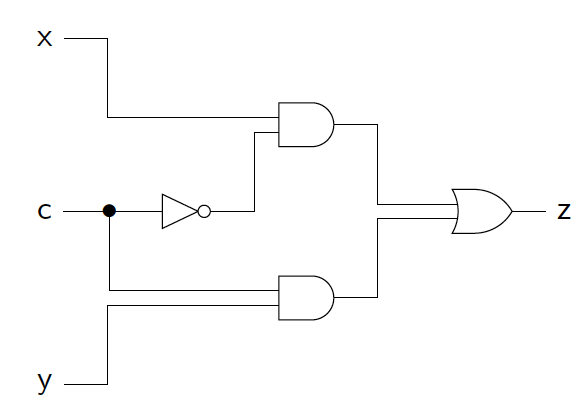
\includegraphics[width=\linewidth]{mux.png}
          \end{figure}
      \end{minipage}
      \hspace{0.05\linewidth}
      \begin{minipage}{0.45\linewidth}
      \begin{tabular}{|c|c|c|c|}
		$c$ & $x$ & $y$ & $z$  \\
		\hline
		$1$ & $1$ & $1$ & $1$ \\
		$1$ & $1$ & $0$ & $0$ \\
		$1$ & $0$ & $1$ & $1$ \\
		$1$ & $0$ & $0$ & $0$ \\ 
		$0$ & $1$ & $1$ & $1$ \\ 
		$0$ & $1$ & $0$ & $1$ \\
		$0$ & $0$ & $1$ & $0$ \\ 
		$0$ & $0$ & $0$ & $0$ \\
	\end{tabular}
	\end{minipage}
\end{minipage}

\newpage
\item \textbf{Demultiplexer}

	\defn{~\label{primitive:dmux}}{The opposite of a multiplexer, it takes a single input converts it into several outputs. It its used to select where to send the input data}
	
	\rem{For $2^n$ possible outputs , $n$ selection signals/lines are required (i.e. 1-to-2 dmux  requires 1 control signal)}
	
		\begin{minipage}{\linewidth}
      \centering
      \begin{minipage}{0.45\linewidth}
     
              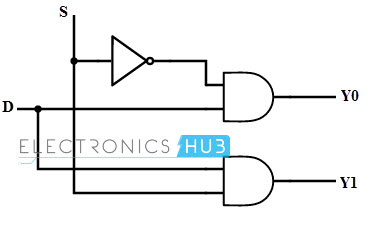
\includegraphics[width=\linewidth]{dmux}
 
      \end{minipage}
      \hspace{0.05\linewidth}
      \begin{minipage}{0.45\linewidth}
      \begin{tabular}{|c|c|c|c|}
		$S$ & $I$ & $Y_1$ & $Y_0$  \\
		\hline
		$0$ & $0$ & $0$ & $0$ \\
		$0$ & $1$ & $0$ & $1$ \\
		$1$ & $0$ & $0$ & $0$ \\
		$1$ & $1$ & $1$ & $0$ \\ 
	\end{tabular}
	\end{minipage}
\end{minipage}
	
	\item \textbf{Half-Adder}
	
	\defn{}{Adds two bits using a 2-bit (carry,sum) representation.}
	
	\par{Note that there's only a carry if both inputs are 1, hence we represent this by an and2 gate, while the sum can be represented by an xor2}
	
	\begin{minipage}{\linewidth}
      \centering
      \begin{minipage}{0.45\linewidth}
              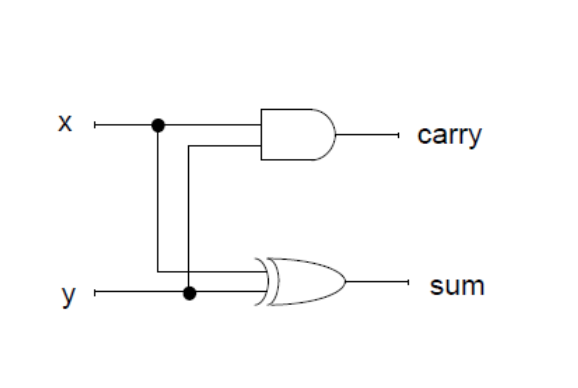
\includegraphics[width=\linewidth]{halfAdder.png}

      \end{minipage}
      \hspace{0.05\linewidth}
      \begin{minipage}{0.45\linewidth}
      \begin{tabular}{|c|c|c|c|}
		$x$ & $y$ & $c (x \land y)$ & $s (x \ \underline{\lor}  \ y)$  \\
		\hline
		$1$ & $1$ & $1$ & $0$ \\
		$1$ & $0$ & $0$ & $1$ \\
		$0$ & $1$ & $1$ & $1$ \\
		$0$ & $0$ & $0$ & $0$ \\ 
	\end{tabular}
	\end{minipage}
	
\end{minipage}

\item \textbf{Full-Adder}
	
	\defn{}{Adds three bits (inputs + carry) using a 2-bit (carry,sum) representation.}
	
	\par{Note that there's only a carry when 2+ inputs are 1, and there's only a sum iff there are an odd number of inputs equal to 1}
	
	\begin{minipage}{\linewidth}
      \centering
      \begin{minipage}{0.65\linewidth}
          
              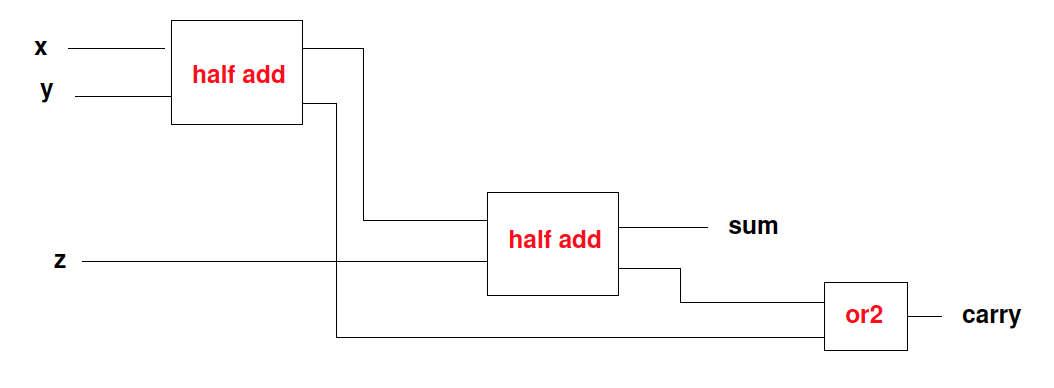
\includegraphics[width=\linewidth]{fullAdder.png}

      \end{minipage}
      \hspace{0.05\linewidth}
      \begin{minipage}{0.25\linewidth}
      \begin{tabular}{|c|c|c|c|c|}
		$x$ & $y$ & $z$ & $c$ & $s$  \\
		\hline
		$1$ & $1$ & $1$ &  $1$ & $1$ \\
		$1$ & $1$ & $0$ &  $1$ & $0$ \\
		$1$ & $0$ & $1$ &  $1$ & $0$ \\
		$1$ & $0$ & $0$ &  $0$ & $1$ \\ 
		$0$ & $1$ & $1$ &  $1$ & $0$ \\ 
		$0$ & $1$ & $0$ &  $0$ & $1$ \\
		$0$ & $0$ & $1$ &  $0$ & $1$ \\ 
		$0$ & $0$ & $0$ &  $0$ & $0$ \\
	\end{tabular}
	\end{minipage}
	
\end{minipage}
\end{enumerate}

\section{Boolean Algebra \& Arithmetics}
\lecture{17}{01}{2019}
\subsection{Laws}

\defn{Idempotence}{operation that can be applied several times without changing the result}

$$ x \lor x = x \quad \quad x \land x = x$$

\defn{Commutative}{operations can be performed in any order}

$$ x \lor y = y \lor x \quad \quad x \land y = y \land x $$

\defn{Associative}{the order in which the operations are performed does not matter as long as the sequence of the operands is not changed}

$$\begin{array} { l } { x \lor ( y \lor z ) = ( x \lor y ) \lor z } \\ { x \land ( y \land z ) = ( x \land y ) \land z } \end{array}$$

\proofs{

\begin{tabular}{lclclclclclclc|}
x & y & z & y $\lor$ z & x $\lor$ y & x $\lor$ (y $\lor$ z) & (x $\lor$ y) $\lor$ z \\
\hline
1 & 1 & 1 & 1 & 1 & 1 & 1 \\
1 & 1 & 0 & 1 & 1 & 1 & 1 \\
1 & 0 & 1 & 1 & 1 & 1 & 1 \\
1 & 0 & 0 & 0 & 1 & 1 & 1 \\
0 & 1 & 1 & 1 & 1 & 1 & 1 \\
0 & 1 & 0 & 1 & 1 & 1 & 1 \\
0 & 0 & 1 & 1 & 0 & 1 & 1 \\
0 & 0 & 0 & 0 & 0 & 0 & 0
\end{tabular}
}

\defn{Distributive \& Absorption}

$$\begin{aligned} x \land ( y \lor z ) & = ( x \land y ) \lor ( x \land z ) \\ x \lor ( y \land z ) & = ( x \lor y ) \land ( x \land z )\end{aligned} $$
$$\begin{aligned} x \land ( x \lor y ) & = x \\ x \lor ( x \land y ) & = x \end{aligned}$$

\rem{Useful for prove of correctness}


\subsection{Arithmetic: Adding 2 Integers}

\defn{4-bit Ripple Carry Adder}{Uses 4 full adders to add two 4-bit numbers}

\begin{figure}[ht]
\centering
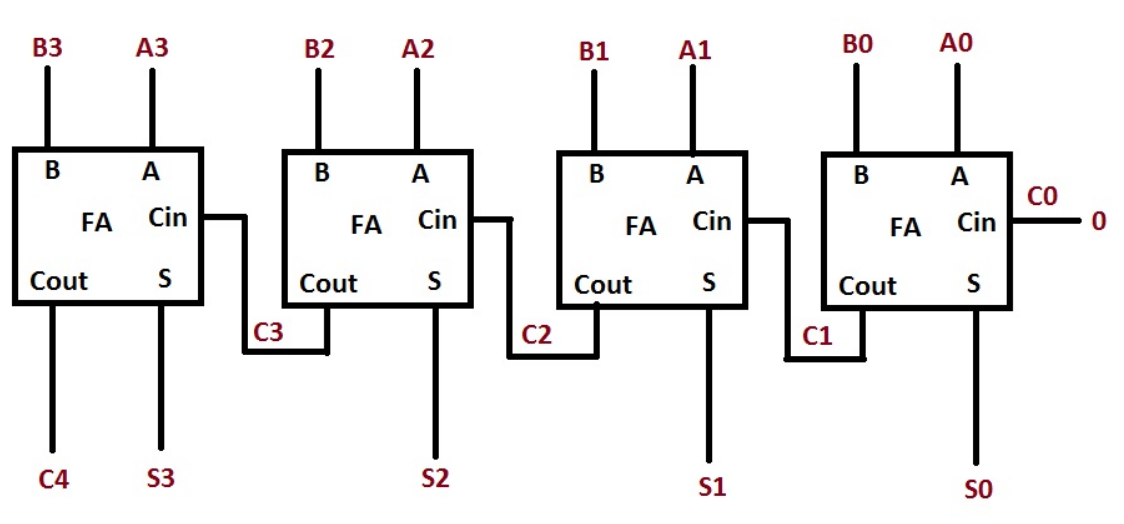
\includegraphics[width=0.7\textwidth]{rippleAdder.png}
\end{figure}

\rem{Note how the carry from each previous operation is passed onto the next, just like how one does addition manually}

\rem{Subtraction can be done much in the some way, by first applying 2's c to one of the inputs}


\section{Synchronous Circuits}

\par{Given that logic gates are physical devices, there is a time delay between an input change and the new output. This makes the circuit stop obeying the boolean laws}

\rem{the clock running faster than it should may lead to invalid outputs, but if it is running slower it simply leads to loss of computational performance/speed}

\rem{Even though the time delay for a gate is marginal, for a whole circuit the delays add up}

\defn{Gate Delay}{Time taken for a gate to respond to a change of input with the correct output}

\ex{ \begin{figure}[ht]
\centering
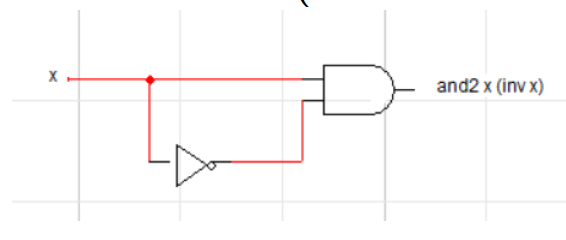
\includegraphics[width=0.5\textwidth]{gateDelay}
\end{figure}

\par{The expected output of the following circuit would be $0$, however when changing from, $1 \text{ to } 0$, the delay of the \code{inv} gate will cause both inputs of the and gate to be $1$, which in turn will erroneously output a $1$ }}

\defn{State}{The stored contents of the memory elements of a circuit, at a given point in time, is collectively referred to as the circuit's state and contains all the information about the past to which the circuit has access}

\defn{Delay Flip Flop (dff)}{component which endows a circuit with state. It has 2 inputs (saved value, clock tick) and 1 output (state value)}

\par{\textbf{Every time} the \code{ dff} receives a clock signal, it updates its state value~\mymarginpar{There is only one clock signal for all flip flops, hence they are all updated simultaneously}. Since the physical components deal with analogue signals, the \ita{clock tick} can not be represented discretely. The workaround is to have the \code{ dff} treat the voltage spike as the tick}

\rem{The output of a \code{ dff} is independent of its input}


\begin{minipage}{\linewidth}
      \centering
      \begin{minipage}{0.45\linewidth}
          
              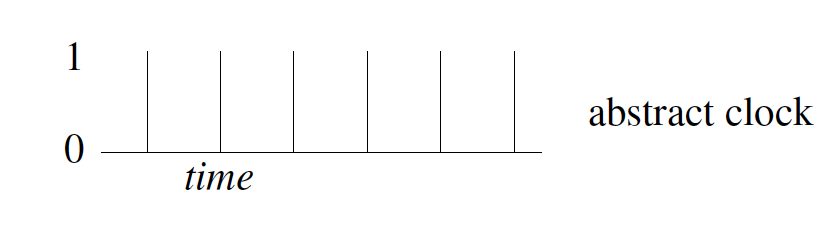
\includegraphics[width=\linewidth]{clock}

      \end{minipage}
      \hspace{0.05\linewidth}
\begin{minipage}{0.45\linewidth}
          
              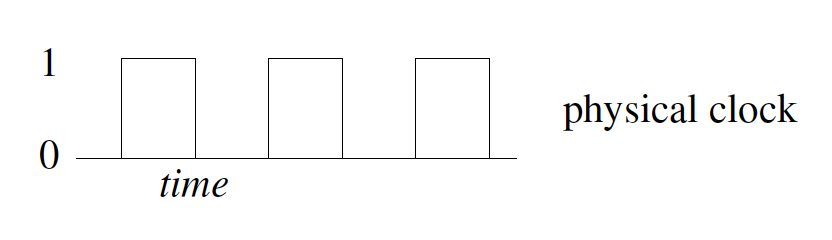
\includegraphics[width=\linewidth]{clock2}

      \end{minipage}
\end{minipage}


\defn{Synchronous Circuit}{
	\begin{enumerate}
		\item Every flip flop must be directly connected to a global clock
		\item No logical functions can be applied to the clock signal
		\item Every clock tick much reach all flip flops simultaneously
		\item Every feedback loop must pass through a flip flop
		\item The inputs to the circuit remain stable throughout clock cycles~\mymarginpar{The cycle must be long enough to allow for all signals to become valid}
	\end{enumerate}
}


\par{At every clock tick the \code{  dff} state gets updated, in order to store its state for longer we can use a register (\code{reg1}). If the control input is 1, then the value from the \code{ dff} is loaded into the \code{ reg1} otherwise it remains the same. The conditional is implemented by an \code{ mux1}}

\defn{Register~\label{primitive:reg}}{Allows the bit to be recorded between cycles, until a new value is loaded. It takes 2 inputs (\code{ ld =1,0} and the value bit) and it outputs the state bit}

\begin{figure}[ht]
\centering
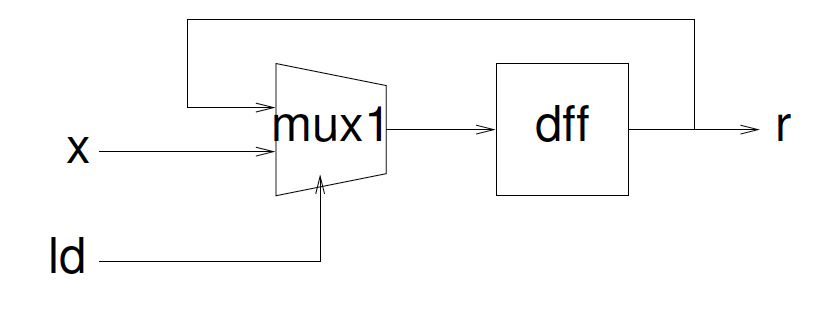
\includegraphics[width=0.7\textwidth]{reg1}
\end{figure}

$$\code{ dff\_input = mux1 ld old\_state x}$$

\par{The register can be simulated by way of a simulation table: }

$$
\begin{tabular}{|c|c|c|c|c|}
	Cycle & \multicolumn{2}{r|}{Inputs}{} & State & Internal \\
	\hline
	& ld & x  & r & dff\_input \\
	\hline
	0 & 1 & 1 & ? & \textbf{1} \\
	1 & 1 & 0 & \textbf{1} & \underline{0}\\
	2 & 0 & 1& \underline{0} & \textbf{0}  \\
	3 & 1 & 1 & \textbf{0} & 1 \\ 
\end{tabular}$$

\section{Register Transfer Machine}

\lecture{25}{01}{2019}

\par{The purpose of an RTM is to use the memory provided by the registers we've learned about in the last lecture to allow simple assignment statements to memory and arithmetic operations to be carried out. To be able to achieve this in a digital circuit, we'll need (1) simple statements (2) A small number of types of statement with a fixed form}

\defn{Opcode}{portion of a machine language instruction that specifies the operation to be performed}

\defn{Instruction}{a group of several bits in a computer program that contains an opcode and usually one or more memory addresses}

\nota{ Assignment \code{ x := y}}

\ex{ Performing an assignment operation, between the value $2$ and the Register 1:
$$ \code{R1 := 2}$$}

\subsection{Register File}

\defn{Register File}{Array of registers (\ref{primitive:reg})}

\par{The register file circuit enables the user to:}
\begin{enumerate}
	\item Specify, address and read out a specific register
	\item Specify and load a value into a new address
\end{enumerate}

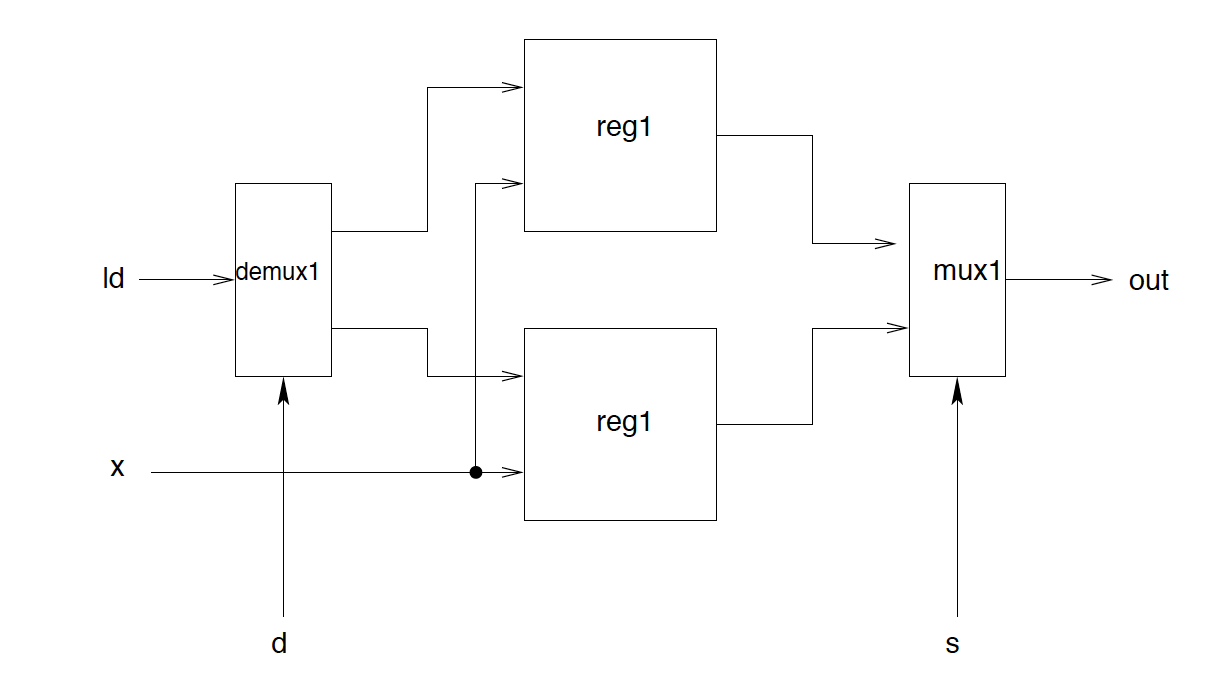
\includegraphics[width=\textwidth]{regFile}

\par{\textbf{Inner Workings}}
\begin{itemize}
	\item The operation to be performed is controlled by \ita{control signals}. These include:
		\begin{itemize}
			\item the "on"/"off" signal or the "load" signal \code{ld}
			\item the memory addresses to the individual registers \code{d, s}
			\item "read"/"write"
		\end{itemize}
		
	\item The input passed onto the circuit \code{x} is loaded into one of the registers \textbf{only} when a clock tick occurs \textbf{and} if \code{ld =1}.
	\item During the cycle select operations may occur, and in the end data is output from a specific register using a memory address passed as another control signal \code{s} 
\end{itemize}

\rem{Note that only the register at address \code{d} will be modified, since the demultiplexer (\ref{primitive:dmux}) will make sure that any other register will have a load control of $0$}

\rem{Note also that since a \code{dmux} (\ref{primitive:dmux}) is able to generate $2^n$ outputs from $n$ inputs, it follows that for controlling a $k$ bit register only $\sqrt{k}$ address bits are required}

\rem{When more than one address needs to be read out, we can pass more source addresses  (\code{s1 s2 s3}) into the multiplexer}

\subsection{RTM Circuit}

\par{Note that the register file allow us to update and read values from inputs, but our intention is to also be able to perform simple arithmetic operations on the values in the registers. This can be done by connecting an adder and a register file in a feedback loop, i.e. the $n$ outputs of the register file, become the $n$ inputs of the adder}

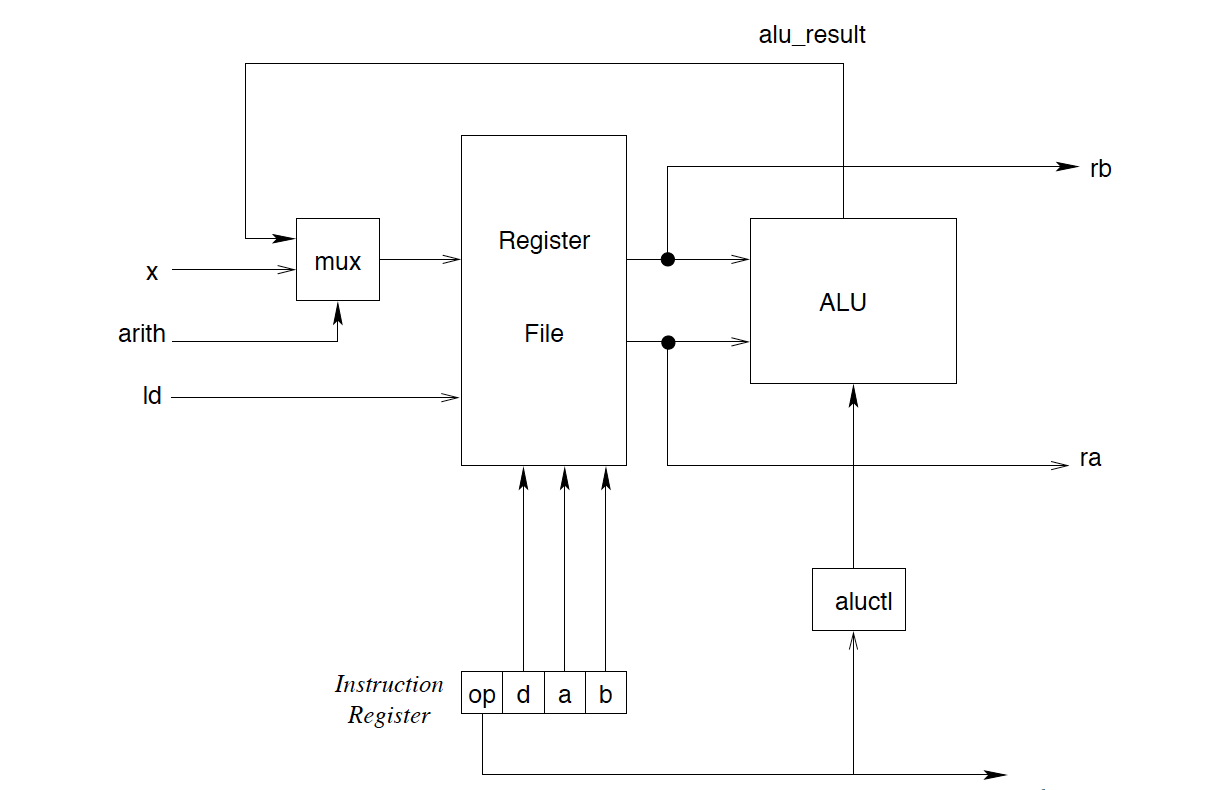
\includegraphics[width=\textwidth]{rtm}

\newpage
\par{\textbf{Inner Workings}}
\begin{itemize}
	\item A multiplexer is added, which allow the user to decide wether to pass onto the register a new value or to pass the result from the adder (hence the feedback)
	\item If the select signal is on \code{arith = 1}, then the file register circuit loads into the register \code[d] the result of the adder in the way describe above
	\item Otherwise, it simply loads the new external output
\end{itemize}

\begin{lstlisting}
if ld 
    then if arith
        then reg[d] := reg[sa] + reg[sb]
        else reg[d] := x
\end{lstlisting}

\par{So now we have a 3rd useful feature provided by the RTM ( on top of the 2 previously seen provided by the register), the possibility of adding two numbers \ita{in memory}. So the following is now possible~\label{rtm:inst}:}

\begin{enumerate}
	\item{Assign an external input to a register \code{R[address] = constant}}
	\item{Adding (or subtracting) two values in memory \code{R[a] = R[b] + R[c]}*\mymarginpar{the two values being added can be from the same register R[a] = R[b] + R[b] or R[a] = R[a] + R[b]}}
\end{enumerate}


\rem{Note however that the following is not possible \ita{within one cycle} \code{R[a] = c + R[b]}, since \code{c} is not in memory}


\newpage
\section{Computer Architecture}
\lecture{29}{01}{2019}
\defn{Computer Architecture}{Defines the structure and the machine language of a computer}

\rem{ Computer Systems' Abstraction Hierarchy}

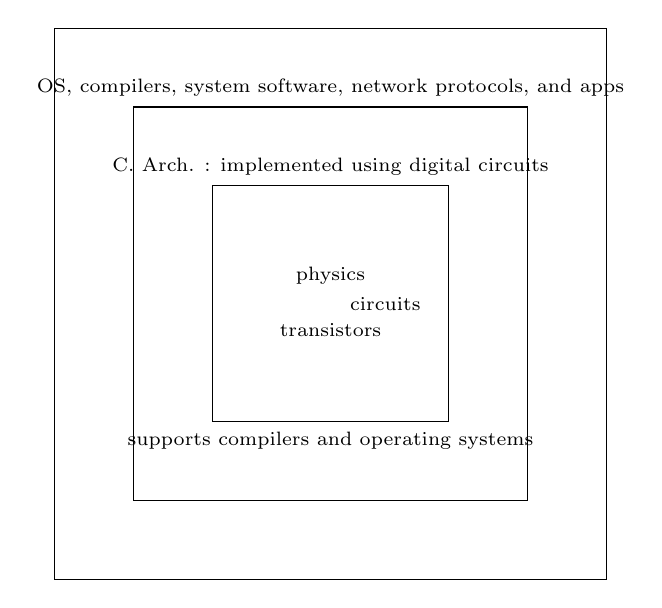
\begin{tikzpicture}
\node[rectangle,draw,
minimum size=7cm]
at (0,0) {};
\node[rectangle,draw,
minimum size=5cm,
label=90:{\scriptsize OS, compilers, system
software, network protocols, and apps}]
at (0,0) {};
\node[rectangle,draw,
minimum size=3cm,
label=90:{\scriptsize C. Arch. : implemented using digital
circuits}, label=-90:{\scriptsize supports compilers and operating systems}]
at (0,0) {};
\node[rectangle,draw=white,
minimum size=0cm, label=90:{\scriptsize physics},
label=-90:{\scriptsize transistors}, label=0:{\scriptsize circuits}]
at (0,0) {};
\end{tikzpicture}

\subsection{Machine Language}

\defn{Machine Language}{The language made up of binary-coded instructions that is used directly by the computer}

\ex{ 
\code{01010000 : operation specifier \\ (4-bit opcode , 1-bit register specifier , 3-bit addressing mode specifier) }\\
\code{0000000001001000 : operand (\$0048 = char "H")}
}

\rem{Each CPU has its own machine language}

\par{High-Level programming languages are \ita{compiled} (converted) into machine language by a compiler. This has the obvious advantage of making programming languages extremely versatile, since one language can be used across many machines, as long as a compiler for it exists }

\defn{Compiler}{Software responsible for translating HLL (nowadays) directly into ML}

\par{The first abstraction from ML was what is know as an \ita{assembly language}, where letter codes represent instructions, instead of bits.}

\defn{Assembly Language}{A low-level programming language in which a mnemonic
represents each of the machine-language instructions for a particular computer}

\defn{Assembler}{Translates AL into ML}

\rem{For this course we'll use a research architecture developed at the university : \code{Sigma16}}

\begin{itemize}
	\item[] \code{Sigma16} features:
	\begin{enumerate}
		\item it has only 16 16-bit registers
		\item uses reduced instruction set
	\end{enumerate}
\end{itemize}

\subsection{Main Subsystems}

\subsubsection{Register File}

\par{There are $16$ , $16$-bit registers. The register file is a volatile memory, used for storing variables for easy access like intermediate values in a calculation }

\nota{\code{Rn} represents the register \code{n}}
\nota{\code{\$0000} represents the data to be stored in \code{hex}}

\rem{\code{R0} is reserved for the number $0$ , and \code{R15} for additional transient information (e.g. overflow?)}

 
 \subsubsection{Arithmetic Logic Unit - ALU}
 
 \defn{ALU}{the circuit that performs arithmetic operations and logical operations (comparison)}
 
 \subsubsection{Memory}
 
 \defn{Memory}{large collection of words}
 
 \par{The memory is much larger (65,536 addresses) and slower, and no arithmetic takes place in it. Instead, it is used for long-term storage.}
 
 \subsection{Input/Output - I/O}
 
 \defn{Input Unit}{A device that accepts data to be stored in memory}
 
 \defn{Output Unit}{A device that prints, displays data or copies it to another device}
 
 \subsection{RTM Instructions}
 
  \par{Remember from above (\ref{rtm:inst}) that the RTM was able to do two things (1) add two numbers; (2) store a number. The following instructions , are how this can be done in  \code{Sigma16}}
  
  \newpage
  \begin{enumerate}
  	\item \textbf{Arithmetic:} \code{op Rst, Rvar1, Rvar2} $\implies$ \code{Rst := Rvar1 op Rvar2}
	
	\nota{ \code{add , sub , mul , div}}
	\ex{
	\code{add R1,R2,R3 ; R1 := R2 + R3}}
	\rem{Note that the \code{;} is used to terminate a sentence, everything after it, in the same line is a comment}
	
	\item \textbf{Memory Access:}
		\begin{itemize}
			\item \code{load Rn, x[R0]} copies \code{x} from memory into \code{Rn}
			\item \code{store Rn, x[R0]} copies the word in \code{Rn} into the var \code{y} in memory
			\item \code{lea Rn, 23[R0]} loads a constant into \code{Rn}
		\end{itemize}
		
		\rem{Note that usually the storage address is the first "argument" but when storing this is reversed}
		
	\item \textbf{Execution:} \code{trap R0,R0,R0} halts the program
	
	\item \textbf{Variable Definition:} \code{x data 98} creates a variable \code{x} with an initial value of $98$
	
	\rem{\code{data} statements must come after all the instructions in the program} 	
\ex{A program that adds two integers: \label{program:add}}

\begin{lstlisting}
load R1,x[R0] ; R1 := x
load R2,y[R0] ; R2 := y
add R3,R1,R2 ; R3 := x + y
store R3,z[R0] ; z := x + y
trap R0,R0,R0 ; terminate

;

x data 23
y data 14
z data 99
\end{lstlisting}

\end{enumerate}

\newpage
\section{Control Structures}
\lecture{31}{01}{2019}

\defn{Control Structures}{Statements that control the flow of execution}

\begin{itemize}
	\item{Conditionals}
	\item{Loops}
	\item{Structuring Computation: functions, recursion, procedures}
\end{itemize}

\subsection{Low Level Constructs}

\par{The \code{jump <label>} statements transfer control to the line of code with the label passed. In \code{Sigma16} there are also two \ita{conditional} jump instructions}

\begin{itemize}
	\item[]\code{ jumpf R1 , <label>[R0]} = if R1 is false, goto label
	\item[]\code{ jumpt R1 , <label>[R0]} = if R1 is true, goto label
\end{itemize}

\rem{Labels must start with a letter, and must be at the beginning of the line}

\par{We can compare expressions using the following:}

\begin{itemize}
	\item[]\code{cmplt R1 R2} ; returns true if R1 $<$ R2
	\item[]\code{cmpeq R1 R2} ; returns true if R1 = R2	
	\item[]\code{cmpgt R1 R2} ; returns true if R1 $>$ R2
\end{itemize}

\subsection{Compilation Patterns}

\par{It is easier to translate high-level languages into machine language, if it is done as a two-step process:}
\begin{enumerate}
	\item Translate complex statements to pseudo-code
	\item Translate pseud-code to machine language
\end{enumerate}

\ex{ Translating \ita{if $x<y$ then a = 1 else a = 2} }

\textbf{1.Pseudo}

\begin{lstlisting}
R3 := (x<y) ; assign boolean to R3
jumpf R4, else[R0] ; jump to label "else" if false
a := 1 ;
jump halt[R0]; jump to label "halt"
else a := 2;

halt trap R0 R0 R0; halt
\end{lstlisting}

\mymarginpar{See slides for more examples of common idioms}

\textbf{2.Low Level}
\begin{lstlisting}
lea R1, 10[R0] ; 
store R1, x[R0] ; 

lea R2, 5[R0] ;
store R2, y[R0] ;

load R1, x[R0] ;
load R2, y[R0];
cmplt R3, R1,R2 ; R3 := (x<y)

jumpf R3, else[R0] ;

lea R4, 1[R0];
store R4, a[R0];

jump halt[R0];

else lea R4, 2[R0];
store R4, a[R0];

halt trap R0 R0 R0;

\end{lstlisting}

\section{Stored Program Computer}
\lecture{05}{02}{2019}
\defn{SPC}{Both the program and the data are stored in the main memory}

\par{In \code{Sigma16} there are 3 types of instructions, each with its own standard format\mymarginpar{The third will covered in future lectures}}

\defn{Instruction Format}{systematic way to represent an instruction using a string of bits}

\subsection{Machine Language}

\rem{Hexadecimal is used to represent each field}

\subsubsection{RRR}

\par{RRR instructions consist of 1 operation and 3 register operands (destination + operands). The assembler reserves 4bits for each field, so that one instruction has a total of 16bits = 1word}

\nota{Standard Names}{\begin{itemize} 
\item[] op : op-code
\item[] d   : destination register address
\item[] a   : operand register address 1
\item[] b   : operand register address 2
\end{itemize}
}

\ex{ \code{add R13,R6,R9} becomes \code{0d69}}

\subsubsection{RX}

\par{RX instructions consist of 1 register - \ita{destination register} - and a memory location composed of the "label" used for the address - \ita{displacement} - and the \ita{index register}}

\par{2 words are needed to represent it: the first has the 4 standard fields and the second contains the displacement}

\ex{Let \code{x} be at the memory address \code{0008}, then \code{load R1,x[R0]} becomes \code{f101 0008}}

\rem{In this case \code{f} is always used as op and \code{b} indicates which operation is being executed}

\subsection{Assembler: Memory Allocation}

\begin{enumerate}
\item The assembler keeps track of where to put the next line of code, by maintaining a variable with a 0-based index - \ita{location counter}
\item It reads each line of code , if a label is value it maps onto the current location and stores it in the \ita{symbol table}; it also decides how many memory an instruction requires and \ita{adds this to the counter}
\item Reads the program a second time
\item Generates the code for each statement, looking up the stored value for labels when needed
\end{enumerate}

\subsubsection{Adder Program (\ref{program:add}) in ML}
\begin{table}[ht]
\begin{center}
\begin{tabular}{|c|c|c|}
address & contents & Meaning \cr
0000 & f101 & first word of load R1,x[R0] \cr
0001 & 0008 & second word: address of x \cr
0002 & f201 & first word of load R2,y[R0] \cr
0003 & 0009 &  second word: address of y \cr
0004 & 0312 & add R3,R1,R2 \cr
0005 & f302 & first word of store R3,z[R0] \cr
0006 & 000a & second word: address of z \cr
0007 & d000 & trap R0,R0,R0 \cr
0008 & 0017 & x = 23 \cr
0009 & 000e & y = 14 \cr
000a & 0063 & z = 99 \cr
\end{tabular}
\end{center}
\end{table}%

\subsection{Control Registers}

\par{CR are registers which the machine uses to keep track of what it is doing, but which are usually not accessible in the program}

\defn{Program Counter}{contains the address of the next line to be executed}

\defn{Instruction Register}{contains the instruction being executed}

\defn{Address Register}{for RX only; contains the address of the second operand}


\section{Arrays}
\lecture{07}{02}{2019}

\defn{Data Structure}{Larger data entity composed of many smaller individual entities \ita{(e.g. arrays, dictionaries, etc.)}}

\defn{Array/Vector}{sequence of indexed values}

\nota{x[i] represents the $i^{th}$ element of the x array}

\par{Arrays can be represented in a computer by placing its elements in consecutive memory locations. The address of the array is equal to that of its first element \code{x[0]}. Every other element can be found by simple \ita{address arithmetic}, i.e. $$\code{x[i] = x+i}$$}

\nota{Defining the array:}

\begin{lstlisting}
; only x[0] has a label
x    data    13   ; x[0]
      data    189 ; x[1]
\end{lstlisting}

\subsection{Indexed Addressing}

\par{Since the address of the array is given by the element at index $0$, a given element is accessed by its \ita{effective address}: the displacement value is added to the index register}

\ex{ \code{x[R4]} where \code{x} represents the address of the element labeled \code{x} - \ita{displacement}; \code{R4} is the \ita{index register}}

\rem{This is the reason why \code{[R0]} is used for simple variables}

\defn{Addressing Mode}{scheme for specifying the address of data \ita{(e.g. displacement[index])}}

\ex{Using Effective Addresses \code{x[i] := x[i] + 50}}

\begin{lstlisting}
lea    R1,50[R0]   ; R1 := 50
load  R5,i[R0]      ; R5 := i
load  R6,x[R5]     ; R6 := x[i]
add   R6,R6,R1   ; R6 := x[i] + 50
store R6,x[R5]     ; x[i] := x[i] + 50
\end{lstlisting}

\subsection{Array Transversal \& For Loops}

\ex{!!!ADD COMPLETE PROGRAM INSTEAD!!!}


\section{Records and Pointers}
\lecture{12}{02}{2019}

\subsection{Compilation Patterns}

\par{Patterns make it easier to translate common idioms. When trying to perform a common task, all one needs to do is pay attention at (1) what common fixed parts you can reuse (2) what varies, i.e. what is specific to the task}

\ex{While Loop}

\begin{lstlisting}
; < >  changeable parts

; High level

    while <bool> do
    	<S>
	
; Low Level Pattern

	label1
	    if <bool> = False goto label2
	    	<Statement>
		goto label1
	label2
\end{lstlisting}

\subsection{Pointers}

\par{Pointers are a sort of "variable", which hold the address of an object. There are two operators, one which returns the address and the other which returns the value of the object}

\nota{Pointer : \&}
\nota{Pointer's Value : *}

\code{lea R5,x[R0] ; R5 := \&x ; address of x is stored in R5}

\code{load R5,x[R0] ; R5 := *x ; value at address [x + 0] stored in R5}

\subsubsection{Comparing accessing a variable directly vs by pointer}

\begin{lstlisting}
; directly

lea R1,5[R0] ; R1 := 5 (constant)
load R2,x[R0] ; R2 := x
add R2,R2,R1 ; R2 := x + 5
store R2,x[R0] ; x := x + 5

; pointer

; R3 := &x
lea R3,x[R0] ; R3 := &x

; Add 5 to whatever word R3 points to
lea R1,5[R0] ; R1 := 5 (constant)
load R4,0[R3] ; R4 := *R3
add R4,R4,R1 ; R4 := *R3 + 5
store R4,0[R3] ; *R3 := *R3 + 5
\end{lstlisting}

\subsection{Records}

\par{Records are essentially an array where every entry is labeled. You can think of it as equivalent to a python dictionary. Each entry can be accessed directly, but the easiest way is to write a block of code using pointers, which can then be reused for all entries}

\ex{ Given a record labeled from A to C}

\begin{lstlisting}
; Set x as the current record by making R3 point to it
lea R3,x[R0] ; R3 := &x

; Perform the calculation on the record that R3 points
load R1,1[R3] ; R1 := (*R3).B
load R2,2[R3] ; R2 := (*R3).C
add R1,R1,R2 ; R1 := (*R3).B + (*R3).C
store R1,0[R3] ; *R3.A := (*R3).B + (*R3).C
\end{lstlisting}

\subsection{Requestes to OS}

\par{Many operations cannot be perform directly by a user program, the main reason being that this would compromise the system's integrity. In order to perform those "sensitive" operations \ita{(e.g. kill exec, read/write, memory allocation, etc)} there are instructions reserved which transfer control to the OS}

\rem{The specific codes used to make a request are defined by the OS, not by the hardware. This is the main reason of why compiled programs are not compatible across systems}


\begin{itemize}
	\item[]Termination : \code{trap R0 R0 R0}
	\item[]Write : \code{trap R1 R2 R3}
		\begin{itemize}
		\item R1 :  the code that indicates a write request
\item R2 : address of the first word of string to write
\item R3 : the length of string
		\end{itemize}
\end{itemize}

\begin{lstlisting}
;To write a string named out, we use (1) lea to load a constant, (2) lea to load the address of an array, (3) load to get a variable

; write out (size = k)
lea R1,2[R0] ; trap code: write
lea R2,animal[R0] ; address of string to print
load R3,k[R0] ; string size = k
trap R1,R2,R3 ; write out (size = k)
trap R0,R0,R0 ; terminate
k data 4 ; length of animal

; animal = string "cat"
animal
data 99 ; character code for 'c'
data 97 ; character code for 'a'
data 116 ; character code for 't'
data 10 ; character code for newline
\end{lstlisting}


\section{Procedures and Call Stack}
\lecture{14}{02}{2019}

\defn{Procedure}{Block of code that performs common tasks}

\par{Instead of repeating code we can write a block of code and call it when necessary by restructuring the flow of the program. Once the procedure finishes the task, the value can be returned and the execution is transferred back to the main flow}

\rem{To avoid breaking the main flow, it is convenient to write the procedure someplace else with a label}

\subsubsection{Implementation}

\par{Note that even though the call is always made to the same place, different calls must return to different places, so it is not possible to just label the caller statement. In order to remember the call origin the statement's address is saved into a register using the \code{jal} instrunction}

\ex{Implementing Call \code{jal R13, fn[R0] ; saves fn address in R13} and Return \code{jump 0[R13]}}

\subsubsection{Passing Parameters}

\rem{By convention, arguments and results are passed in R1}

\begin{lstlisting}
;Main program
load R1,x[R0] ; arg = x
jal R13,work[R0] ; result = work (x)
...
load R1,y[R0] ; arg = y
jal R13,work[R0] ; result = work (y)
...

; Function work (x) = 1 + 7*x
work lea R2,7[R0] ; R7 = 2
lea R3,1[R0] ; R3 = 1
mul R1,R1,R2 ; result = arg * 7
add R1,R3,R1 ; result = 1 + 7*arg
jump 0[R13] ; return
\end{lstlisting}

\subsubsection{Recursive Calls}

\par{Note that if a procedure is called recursively, then registers might be overwritten. In order to execute recursive calls, we need to \ita{save the state} of the caller. This can be achieved, by using a \ita{call stack}}

\defn{Stack}{Data container which only supports \ita{push} and \ita{pop}, hence at any given time, only the top element is accessible}

\par{Because most procedures usually need several registers, recursive calls would quickly exhaust the number of available registers. Hence the state needs to be saved in memory:}

\begin{enumerate}
	\item At the start of the procedure, there must be a store instruction for its return address \mymarginpar{By convention, R13 will always be used as the return}
	\item At the end of the procedure, the return address must be loaded and passed to jump
\end{enumerate}

\subsubsection{Call Stack}

\defn{Call Stack}{Data container which stores all the information about calls and returns}

\par{Every call triggers the following to be stored in memory:}

\begin{itemize}
	\item[] a pointer to the previous stack frame (needed for pop)
	\item[] the return address
	\item[] the saved registers
	\item[] local variables (frees up working memory for the procedure)
\end{itemize}

\par{We implement the stack by dedicating \code{R14} to the stack pointer , saving the word with the info at \code{0[R14] + 1} at call time, and reseting it when returning. (i.e. \code{0[R14] -1})}

\rem{Note that \code{R14} must remain unchanged, otherwise the pointer to the stack will be overwritten}

\section{Variables}
\lecture{19}{02}{2019}

\par{Variables are distinguished according to 3 features:}
\begin{enumerate}
	\item Lifetime: When it is created and destroyed
	\item Scope: From where it can be accessed
	\item Location: Address in memory
\end{enumerate}

\subsection{Static}

\par{Static Variables are created at the start of the program, and retain their values until the program terminates. The variables defined using the \code{data} instruction, initialized after the trap instruction are static}

\par{To avoid the duplication of instructions, and to allow for executable code to be shared, variables and code are often separated.}

\defn{Code Segment}{Shareable, read-only part of the program}
\defn{Data Segment}{Non-Shareable, read-write part of the program}

\subsection{Local}

\par{Local Variables on the other hand are defined within the program (e.g. within a function, a block etc.). Local variables have only one name, but there may be many instances of it (e.g. recursive calls). Hence, instead of storing them in memory using \code{data}, they are kept in \ita{stack frames}}

\par{Local Variables can be accessed by addressing them \ita{relative} to the stack frame}

\subsection{Dynamic}

\par{Dynamic Variables are created explicitly, and therefore they are not limited to blocks of code, and need not follow the  push-pop order of the stack. Hence, they can neither be kept in the stack frame nor in the static data segment. They are instead kept in the \ita{heap}}

\defn{Heap}{Data structure composed of a very large number of small objects. It contains a \ita{free space list} - a data structure which points to all the free words of memory}

\par{When the variable is created a small chunk of memory from the heap points to the object, once the variable is destroyed the memory pointer is released back into the \ita{free space list}}

\subsection{Call Stack}

????



\newpage

\section{Linked Lists}

\defn{Linked List}{Linear chain of nodes}

\defn{Node}{Record with two fields: (1) \ita{value} - word containing info (2) \ita{next} - pointer to the next node}

\rem{The last element of a linked list has \ita{value} $=$ \ita{nil}}

\par{As seen above, we can access the fields of a record using pointers' arithmetic. Hence, for a given pointer \code{p}}

\begin{lstlisting}
; load the pointer to the node into R1
load R1,p[R0] ; R1 := p 
; load the value field at position 0 into R2
load R2,0[R1] ; R2 := (*p).value 
; load the next field at position 1 into R3
load R3,1[R1] ; R3 := (*p).next 
\end{lstlisting}

\par{

\subsection{Basic Operations}

\rem{Assuming that \code{p,q} are in memory. Normally, these will be kept in registers so as to minimize the number of \code{load,store} instructions}

\subsubsection{Is Empty?}

\begin{lstlisting}
load R1,p[R0]
cmpeq R2,R1,R0
jumpt R2,pIsEmpty[R0]
; Not empty Body
...
; Empty Body
pIsEmpty ...
\end{lstlisting}

\subsubsection{Return Value}
\begin{lstlisting}
load R1,p[R0] ; R1 := p
load R2,0[R1] ; R2 := *p.value
store R2,x[R0] ; x := *p.value
\end{lstlisting}

\subsubsection{Return Next}
\begin{lstlisting}
load R1,p[R0] ; R1 := p
load R2,1[R1] ; R2 := *p.value
store R2,q[R0] ; q := *p.value
\end{lstlisting}

\rem{Nothing new! Just like accessing a record,\code{value} has an offset of 0 and \code{next} has an offset of 1}

\subsection{Transversing}

\par{Using a while loop, with the stoping condition of \ita{pointer} $\neq 0 $. Since the last element of the list is nil}

\subsection{Cons}

\defn{Cons}{A term from functional languages. To \ita{cons x onto y} loosely means to create a new object from y by "appending" an object x of the same type}

\ex{ Given a list \code{p = [1,2]} , \code{q = [3,1,2] ; cons(3, p)}}

\begin{lstlisting}
cons (x, p)
	{ q := newnode ();
	(*q).value := x;
	(*q).next := p;
	return q;
	}
\end{lstlisting}

\rem{Note that p is unchanged. A new node is created, which points to p with the new added value}

\mymarginpar{memory management too detailed?}

\subsection{Lists Vs Arrays}

\begin{table}[htp]
\begin{center}
\begin{tabular}{|c|c|c|}
Feature & Array & List \\
\hline
\textbf{Direct Element Access} & Yes (with arbitrary index) & No (only to element with pointer) \\
\hline
\textbf{Traversing} & Yes (for loop i++) & Yes (set pointer to p.next, until p is nil) \\
\hline
\textbf{Memory p/el} & = element & = el + node \\
\hline
\textbf{Flexibility} & Fixed \& Fully Allocated & Variable \& Dynam Allocated \\
\hline
\end{tabular}
\end{center}
\end{table}

\subsection{General Data Structures}

\par{By using more pointers, more general structures can be created. For example: (1) Double Linked List (points back-forward) (2) Circular (no nill valued node)}

\subsection{Abstract Data Type}

\defn{ADT}{A data type defined by its behaviour (semantics) , i.e. the operations it supports. Thought of from the point of view of the user instead of the implementer}

\par{An example of this type of structure is a stack. The core idea behind it is to support "push-pop" of data, but it can be implemented in more than one way, depending on what is required by the program. For example, instead of array, a linked list can be used:}

\begin{lstlisting}
; List Stack

Empty stack as nil
Push x is implemented by stack := cons (x, stack)
Pop x is implemented by stack := (*stack).next

; Array Stack

; PUSH
; stack[stTop] := R1; stTop := stTop + 1

push load R1,x[R0] ; R1 := x
load R2,stTop[R0] ; R2 := stTop
store R1,stack[R2] ; stack[stTop] := x
lea R3,1[R0] ; R3 := constant 1
add R2,R2,R3 ; R2 := stTop + 1
store R2,stTop[R0] ; stTop := stTop + 1

; POP

; pop the stack, store top element into x
; stTop := stTop - 1; x := stack[stTop]

pop load R2,stTop[R0] ; R2 := stTop
lea R3,1[R0] ; R3 := constant 1
sub R2,R1,R3 ; R2 := stTop - 1
load R1,stack[R2] ; R1 := stack[stTop-1]
store R1,x[R0] ; x := stack[stTop-1]
store R2,stTop[R0] ; stTop := stTop - 1

\end{lstlisting}

\subsection{Error Checking}

\par{The previous implementation does not check for errors, which might cause the program to crash or to output the wrong data. In order to prevent that, programs need to be able to check and handle errors.}

\begin{itemize}
	\item Error message
	\item Error code to caller, and transfer control
	\item Throw an exception
	\item Terminate Execution
\end{itemize}

\lecture{25}{02}{2019}

\section{Programming Techniques}

\subsection{Compound Boolean Expressions: Short Circuit}

\defn{Short Circuit}{When two conditions need to be satisfied, if the first fails, we can save resources by skipping the evaluation of the second}

\begin{lstlisting}
; while i<n && x[i]>0 do S
; if not (i<n && x[i]>0) then goto loopDone

load R1,i[R0] ; R1 := i
load R2,n[R0] ; R2 := n
cmplt R3,R1,R2 ; R3 := i<n
jumpf R3,loopDone[R0] ; if not (i<n) then goto loopDone
load R3,x[R1] ; R3 := x[i] safe because i<n
cmpgt R4,R3,R0 ; R4 := x[i]>0
jumpf R4,loopDone[R0] ; if not (x[i]>0) then goto loopDo
\end{lstlisting}

\subsection{Condition Code}

\par{Instead of storing the comparison boolean in a register and jump, it is possible to use the instruction \code{cmp} which stores the result - \ita{condition code} - in \code{R15} and then one of the condition jump operators (e.g. \code{jumplt})}

\subsection{Repeat-until Loop}

\begin{lstlisting}
; stopping condition checked at the end

repeat
	{S1; S2; S3}
until i>n;
\end{lstlisting}

\section{Arrays \& Pointers}

\subsection{Accessing Elements with Pointers}

\begin{lstlisting}
lea R1,x[R0] ; point p to first el of array x store in R1
load R2,0[R1] ; access the value p points to store in R2
lea R1,1[R1] ; p++
\end{lstlisting}

\rem{Note that the arithmetic happens on the pointers}

\subsection{Sum}

\begin{lstlisting}
; R1 = p = pointer to current element of array x
; R2 = q = pointer to end of array x
; R3 = sum of elements of array x

	lea R1,x[R0] ; p := &x
	lea R2,xEnd[R0] ; q := %xEnd
	add R3,R0,R0 ; sum := 0
sumLoop
	cmplt R4,R1,R2 ; R4 := p<q
	jumpf sumLoopDone ; if not p<q then goto sumLoopDone
	load R4,0[R1] ; R4 := *p (this is current element of x)
	add R3,R3,R4 ; sum := sum + *p
	lea R1,1[R1] ; p := p+1 (point to next element of x)
	jump sumLoop[R0] ; goto sumLoop
sumLoopEnd

x 	data 23 ; first element of x
	data 42 ; next element of x
	data 19 ; last element of x
xEnd
\end{lstlisting}

\rem{It is easier to use ArraySum with pointers for records}

\subsection{Traverse}

\begin{lstlisting}

; LOW LEVEL

; sum := 0;
; p := &RecordArray;
; q := &RecordArrayEnd;
; RecordLoop
; if (p<q) = False then goto recordLoopDone;
; *p.fieldA := *p.fieldB + *p.fieldC;
; sum := sum + *p.fieldA;
; p := p + RecordSize;
; goto recordLoop;
; RecordLoopDone

; Sigma16

; R1 = sum
; R2 = p (pointer to current element)
; R3 = q (pointer to end of array)
; R4 = RecordSize

	lea R1,0[R0] ; sum := 0
	lea R2,RecordArray[R0] ; p := &RecordArray;
	lea R3,RecordArrayEnd[R0] ; q := &RecordArray;
	load R4,RecordSize[R0] ; R4 := RecordSize
RecordLoop
	cmplt R5,R2,R3 ; R5 := p<q
	jumpf R5,RecordLoopDone[R0] ; if (p<q) = False then goto RecordLoopDone
	load R5,1[R2] ; R5 := *p.fieldB
	load R6,2[R2] ; R6 := *p.fieldC
	add R7,R5,R6 ; R7 := *p.fieldB + *p.fieldC
	store R7,0[R2] ; *p.fieldA := *p.fieldB + *p.fieldC
	add R1,R1,R7 ; sum := sum + *p.fieldA
	add R2,R2,R4 ; p := p + RecordSize
	jump RecordLoop[R0] ; goto RecordLoop
RecordLoopDone
\end{lstlisting}

\subsection{Stack Overflow}

\rem{ \code{R12, R11} registers dedicated to store info for procedures. 12 - \ita{stack top} , 11 - \ita{stack limit}}

\subsubsection{Initialize Stack}
\begin{lstlisting}
lea R14,CallStack[R0] ; initialise stack pointer
store R0,0[R14] ; main program dynamic link = nil
lea R12,1[R14] ; initialise stack top
load R1,StackSize[R0] ; R1 := stack size
add R11,R14,R1 ; StackLimit := &CallStack + StackSize
\end{lstlisting}

\newpage
\subsubsection{Call, Return, Stack Overflow}

\rem{arguments are passed in the first registers}

\begin{lstlisting}

; Create stack frame
store R14,0[R12] ; save dynamic link
add R14,R12,R0 ; stack pointer := stack top
lea R12,6[R14] ; stack top := stack ptr + frame cmp R12,R11 ; stack top ~ stack limit
jumpgt StackOverflow[R0] ; if top>limit then goto stack store R13,1[R14] ; save return address
store R1,2[R14] ; save R1
store R2,3[R14] ; save R2
store R3,4[R14] ; save R3
store R4,5[R14] ; save R4

; return
load R1,2[R14] ; restore R1
load R2,3[R14] ; restore R2
load R3,4[R14] ; restore R3
load R13,1[R14] ; restore return address
load R14,0[R14] ; pop stack frame
jump 0[R13] ; return

; If the stack is full and a procedure is called, this is a fatal error. Error message is printed
; StackOverflow

lea R1,2[R0]
lea R2,StackOverflowMessage[R0]
lea R3,15[R0] ; string length
trap R1,R2,R3 ; print "Stack overflow\n"
trap R0,R0,R0 ; halt

StackOverflowMessage
	data 83 ; 'S'
	data 116 ; 't'
	data 97 ; 'a'
	data 99 ; 'c'
	data 107 ; 'k'
...
\end{lstlisting}

\section{Nested Conditionals}

\lecture{28}{02}{2019}

\subsection{Jump Tables}

\par{A bunch of \ita{if-then} or \ita{case} statements are inefficient if we're looking to match a numeric code directly. This can instead be done by constructing an array made of jumps to certain conditional statements which match the code passed as an argument. A sort of table of "tasks"}

\begin{lstlisting}
; Jump to operation specified by code
add R4,R4,R4 ; code := 2*code
lea R5,CmdJumpTable[R0] ; R5 := pointer to jump table
add R4,R5,R4 ; address of jump to operation
jump 0[R4] ; jump to jump to operation

CmdJumpTable
	jump CmdTerminate[R0] ; code 0: terminate the program
	jump CmdInsert[R0] ; code 1: insert
	jump CmdDelete[R0] ; code 2: delete
	jump CmdSearch[R0] ; code 3: search
	jump CmdPrint[R0] ; code 4: print

CmdDone
	load R5,InputPtr[R0]
	lea R6,3[R0]
	add R5,R5,R6
	store R5,InputPtr[R0]
	jump CommandLoop[R0]
\end{lstlisting} 

\rem{If the code passed does not exist in the table, program will jump to random instruction. Error Check by comparing code with least/largest value in table}

\newpage


\nocite{*}
\printbibliography


\end{document}
